\documentclass[11pt]{article}
\usepackage[sc]{mathpazo} 
\usepackage{fullpage}
\usepackage{natbib}
\linespread{1.5}
\usepackage[utf8]{inputenc}
\usepackage{lineno}
\usepackage{titlesec}
\titleformat{\section}[block]{\Large\bfseries\filcenter}{\thesection}{1em}{}
\titleformat{\subsection}[block]{\Large\itshape\filcenter}{\thesubsection}{1em}{}
\titleformat{\subsubsection}[block]{\large\itshape}{\thesubsubsection}{1em}{}
\titleformat{\paragraph}[runin]{\itshape}{\theparagraph}{1em}{}[. ]\renewcommand{\refname}{Literature Cited}
% my addnl packages
\usepackage{geometry}
\usepackage{graphicx}
\usepackage[T1]{fontenc}
\usepackage{authblk}
\usepackage{setspace}
\usepackage{amsfonts,amssymb,amsmath,hyperref}
\usepackage{float}
\usepackage{caption}
\usepackage{multirow}
\usepackage{hyperref}
\usepackage{wrapfig}
\usepackage{rotating}
\usepackage[usenames,dvipsnames]{xcolor}
\newcommand{\revise}[1]{{\color{Mahogany}{#1}}}
\usepackage[normalem]{ulem}
\graphicspath{{/Users/jm200/Library/CloudStorage/Dropbox/Miller Lab/github/POAR-Forecasting/Manuscript/Figures/}}
\newcommand{\tom}[2]{{\color{red}{#1}}\footnote{\textit{\color{red}{#2}}}}


\doublespacing


%-------------------------------------------------------------------------
\title{Forecasting range shifts of a dioecious plant species under climate change}

\author[1]{Jacob K. Moutouama}
\author[2]{Aldo Compagnoni}
\author[1]{Tom E.X. Miller}
\affil[1]{Program in Ecology and Evolutionary Biology, Department of BioSciences, Rice University, Houston, TX USA}
\affil[2]{Institute of Biology, Martin Luther University Halle-Wittenberg, Halle, Germany; and German Centre for Integrative Biodiversity Research (iDiv), Leipzig, Germany}
%-------------------------------------------------------------------------
\usepackage{Sweave}
\begin{document}
%\SweaveOpts{concordance=TRUE}
\maketitle
\noindent{} $\ast$ Corresponding author: jmoutouama@gmail.com\\
\noindent{} Submitted to \textit{Ecology letters}\\
\noindent{} Manuscript type: Article\\
\noindent{} Open Research statement: All of our data and code are available during peer review at \url{https://github.com/jmoutouama/POAR-Forecasting}. This manuscript and its contents can be reproduced from this file: \url{https://github.com/jmoutouama/POAR-Forecasting/Manuscript/Forescasting.Rnw}. All data are provided at \url{https://github.com/jmoutouama/POAR-Forecasting/tree/main/data}.
%\SweaveOpts{concordance=TRUE}

\linenumbers
%-------------------------------------------------------------------------
\newpage
\section*{Abstract}
Sex-specific response to rising temperature and drought raises the questions of whether global change could lead to a drastic change in the sex ratio and whether that change in the sex ratio could drive population extinction or population range shift in dioecious species.
Answering these questions requires an understanding of the mechanism by which a change in vital rates under future climate conditions for both male and female, could be translated into a significant change in population dynamics.
We forecast range shift for a dioecious species using matrix models. 


%-------------------------------------------------------------------------
\section*{Keywords}
climate change, demography, forecasting, matrix projection model, mechanistic models, sex ratio, range limits

%--------------------------------------------------------------------
\newpage
\section*{Introduction}
Rising temperatures and extreme drought events associated with global climate change are leading to increased concern about how species will become redistributed across the globe under future climate conditions \citep{bertrand2011changes,gamelon2017interactions,smith2024extreme}.
Dioecious species might be particularly vulnerable to the influence of climate change because they often display skewed sex ratios that are generated or reinforced by sexual niche differentiation (distinct responses of females and males to shared climate drivers) \citep{Tognetti2012}. 
Accounting for such a niche differentiation between male and female within a population is a long-standing challenge in accurately predicting which sex will successfully track environmental change and how this will impact population dynamics \citep{jones1999sex,gissi2023exploring}. 
The vast majority of theory and models in population biology, including those used to forecast biodiversity responses to climate change, ignore the complication of sex structure \citep{pottier2021sexual,ellis2017does}.
As a result, accurate forecasts of colonization-extinction dynamics for dioecious species under future climate scenarios are limited. 

Climate change can influence dioecious populations via shifts in sex ratio. 
Females and males respond differently to climate change, especially in species where there is sexual niche differentiation \citep{gissi2023exploring,gissi2023sex,hultine2016climate}. 
This sex-specific response to climate change may help one sex to succeed in extreme climatic conditions more than the other sex leading to a skewness in the operational sex ratio (relative number of males and females who are ready to mate) \citep{eberhart2017sex,zhao2012sex, burli2022environmental} .
Experimentation manipulation revealed that when exposed to increasing temperatures, for example, in two populations of Atlantic marine copepods (\textit{Acartia tonsa}), males showed significantly lower survival than females \citep{sasaki2019complex}.
However, in some species, such as \textit{Pteropus poliocephalus} or \textit {Populus cathayana}, females showed lower survival than males in response to high temperature \citep{welbergen2008climate,zhao2012sex}.

Species's range limits, when not driven by dispersal limitation, should generally reflect the limits of the ecological niche. 
For most species, niches and geographic ranges are often limited by climatic factors including temperature, precipitation \citep{sexton2009evolution}. 
Therefore, any substantial changes in the magnitude of these climatic factors in a given location across the range could impact population viability  with potential implication on range shift \citep{davis2001range, pease1989model}. 
This is particularly true for dioecious species in which each sex has a different sensitivity to climate variation\citep{pottier2021sexual,morrison2016causes}.
Populations in which males are rare under current climatic conditions could experience low reproductive success due to sperm or pollen limitation that may lead to population decline in response to climate change \citep{eberhart2017sex}.
In contrast, climate change could lead to male moving to more suitable areas (e.g. upslope), which might favor range expansion \citep{petry2016sex}.
Although the response of species to warming is generally understood, it is difficult to disentangle the interaction between sex and climate drivers to understand their relative contribution and effect on population dynamics and the consequence of such effect on range  shift. 

Our ability to track the impact of climate change on the population dynamics of dioecious plants and the implication of such impact on range shift depends on our ability to build mechanistic models that take into account the spatial and temporal context in which sex specific response to climate change affects population viability \citep{davis2001range,evans2016towards,czachura2020demographic}.
At their range edge where climatic conditions are expected to be less favorable, if dioecious species populations are non-viable in response to climate change, global warming will induce range contraction in dioecious species.
In reverse, if populations at the edge are viable habitats in response to global warming, dioecious species populations could shift their range and relocate to more favorable and thereby favored range expansion. 

In this study, we used a mechanistic approach by combining field experiment and matrix projection modelling, to understand the demographic response of dioecious species to climate change and its implications for future range dynamics.
Our study system is a dioecious plant species (\textit{Poa arachnifera}) distributed along environmental gradients in the south-central US corresponding to variation in temperature across latitude and precipitation across longitude (MAP). 
% A previous study showed that, despite the differentiation of the climatic niche between sexes, the female niche mattered the most in driving the environmental limits of population viability \citep{miller2022two}. 
Here, we asked three questions: (1) What is the sex-specific demographic response to rising temperature and precipitation ?
(2) How that sex-specific demographic response affects populations dynamics under current and future climatic conditions ?
(3) What are the implications of population dynamics on range dynamics ?   

%--------------------------------------------------------------------
\section*{Materials and methods}

\subsection*{Study species}
Texas bluegrass (\textit{Poa arachnifera}) is a perennial, summer-dormant cool-season (C3) grass. 
The species occurs in Texas, Oklahoma, and southern Kansas, USA \citep{hitchcock1971manual}. 
Texas bluegrass grows during cool months between October and May, with onset of dormancy often from June to September \citep{kindiger2004interspecific}.
Flowering occurs in May and the species is pollinated by wind \citep{hitchcock1971manual}.

\subsection*{Common garden experiment}
We set up a common garden experiment to manipulate climatic factors (e.g.,temperature and precipitation) to detect mechanisms underlying sex-specific demographic response to climate and the implication of such a response on range limitation \citep{merow2017climate,schwinning2022common}. 
At this end, we collected vegetative tillers from flowering individuals of each sex in eight natural (sources) populations of the focal species.
We then propagated these tillers in ProMix plotting soil and supplemented them with Osmocote slow-release fertilizer at $75^\circ$F to $85^\circ$F under natural climatic conditions at the Rice University Greenhouse. 
The common experiment was installed on 14 sites across a precipitation gradient (FigX). At each site, we established 14 blocks. Each block was selected so that they resemble the natural environment of the species. For each block we planted three females and three males individuals. We spared the individuals, provided \~ 1 L  of water, and removed surrounding vegetation to avoid competition and promote establishment. 

\subsection*{Demographic and climatic data collection}
To  parametrize the demographic models, we first collected individual demographic data including survival (alive or dead), growth (number of tillers), flowers (reproductive or vegetative), and fertility (number of panicles) in each site for two censuses (2015 and 2016). 
Secondly, we downloaded monthly temperature and precipitation from Chelsa to describe observed climate conditions \citep{karger2017climatologies}.
These climate data were used as covariates in vital rate regressions, which allowed us to forecast and back-cast the effect of climate change on population dynamics and map species’ niche and distribution under future and past climate change. 
We prefer temperature and precipitation because they capture the most the climate in the study region \colorbox{BurntOrange}{Source}. 
Since our experiment was installed in November, we aligned the climatic years to match demographic transition years rather than calendar years.
Then we used the monthly data to estimate seasonal data (dormant and growing season), since our study species is a seasonal cool grass. 
We define June to September as the dormant season of the year and the rest of the year as the growing season. 
To back-cast and forecast the effect of future climate on species population dynamics, we downloaded climatic projection data for past climatic conditions (901-1930), current conditions (1990-2019) and future conditions (2070-2100).
These climatic conditions (past, present and future) were downloaded from four general circulation models (GCMs) selected from the Coupled Model Intercomparison Project Phase 5 (CMIP5). 
The GCMs are MIROC5, ACCESS1-3, CESM1-BGC, CMCC-CM  and were downloaded from chelsa \citep{sanderson2015representative}.
We evaluated future climate projections from two scenarios of representative concentration pathways (RCPs): RCP4.5, an intermediate-to-pessimistic scenario assuming a radiative forcing to amount to 4.5 $W m^{-2}$ by 2100, and RCP8.5, a pessimistic emission scenario which project a radiative forcing to amount to 8.5 $W m^{-2}$ by 2100 \citep{thomson2011rcp4, schwalm2020rcp8}.

\subsection*{Sex ratio experiment}

We conducted a sex-ratio experiment on a site close (1 km) to a natural population of the focal species at the center of the range to estimate the effect of sex-ratio variation on female reproductive success.
Details of the experiment are provided in \cite{compagnoni2017can} and \cite{miller2022two}.
In short, we established 124 experimental populations on plots measuring 0.4 x 0.4m and separated by at least 15m from each other at that site. 
We chose 15m because our pilot data show that more than 90\% of wind pollination occurred within 13m. 
We varied population density (1-48 plants/plot) and sex ratio (0\%-100\% female) across the experimental populations, and we replicated 34 combinations of density-sex ratios. 
We collected the number of panicles from a subset of females in each plot and collected the number of seeds in each panicle.
Since the number of panicles (proxy of reproduction effort) does not necessarily reflect reproduction success in \textit{Poar arachnifera}, we accessed reproduction success (seed fertilized) using greenhouse-based germination and trazolium-based seed viability assays. 

We used the sex-ratio to estimate the probability of viability and the germination rate. 
Seed viability was modeled with a binomial distribution where the probability of viability ($v$) was given by:
\begin{align}\label{eq:viab_fn}
v = v_{0} * (1 - OSR^{\alpha})
\end{align}
\noindent where $OSR$ is the operational sex ratio (proportion of panicles that were female) in the experimental populations.
The properties of the above function is supported by our previous work \citep{compagnoni2017can}. 
Here, seed viability is maximized at $v_{0}$ as $OSR$ approaches zero (strongly male-biased) and goes to zero as $OSR$ approaches $1$ (strongly female-biased).
Parameter $\alpha$ controls how viability declines with increasing female bias.

We used a binomial distribution to model the germination data from greenhouse trials.
Given that germination was conditional on seed viability,the probability of success was given by the product $v*g$, where $v$ is a function of $OSR$ (Eq. \ref{eq:viab_fn}) and $g$ is assumed to be constant.

\subsection*{Sex specific demographic responses to climate}
We used individual level measurements of survival, growth (number of tillers), flowering, number of panicles to independently develop Bayesian mixed effect models describing how each vital rate varies as a function of sex, size, precipitation of growing and dormant season and temperature of of growing and dormant season. 
We fit vital rate models with second-degree polynomial functions for the influence of climate.
We included a second-degree polynomial because we expected that climate variables would affect vital rates through a hump-shaped relationship. 

We centered and standardized all predictors to facilitate model convergence.
We included site,source, and block as random effect.
All the vital rate models used the same linear and quadratic predictor for the expected value ($\mu$)(Eq. \ref{eq:mu}) . 
However, we applied a different link function ($f(\mu)$) depending on the distribution the vital rate. 
We modeled survival and flowering data with a Bernoulli distribution.
We modeled the growth (tiller number) with a zero-truncated Poisson inverse Gaussian distribution. 
Fertility (panicle count) was model as zero-truncated negative binomial. 
\begin{align}\label{eq:mu}
\begin{split}
f(\mu) = \beta_{0} + \beta_{1}size + \beta_{2}sex + \beta_{3}pptgrow + \beta_{4}pptdorm + \beta_{5}tempgrow + \beta_{6}tempdorm \\ 
+ \beta_{7}pptgrow*sex + \beta_{8}pptdorm*sex + \beta_{9}tempgrow*sex + \beta_{10}tempdorm*sex  \\ 
+  \beta_{11}size*sex + \beta_{12}pptgrow*tempgrow + \beta_{13}pptdorm*tempdorm\\
+ \beta_{14}pptgrow*tempgrow*sex + \beta_{15}pptdorm*tempdorm*sex + \beta_{16}pptgrow^2\\
+ \beta_{17}pptdorm^2 + \beta_{18}tempgrow^2 + \beta_{19}tempdorm^2 + \beta_{20}pptgrow^2*sex  \\
+ \beta_{21}pptdorm^2*sex + \beta_{22}tempgrow^2*sex + \beta_{23}tempdorm^2*sex + \phi + \rho + \nu 
\end{split}
\end{align}
\noindent where $\beta_{0}$ is the  grand mean intercept, $\beta_{1}$...$\beta_{13}$ represent the size and climate dependent slopes.
$size$ was on a natural logarithm scale. 
$pptgrow$ is the precipitation of the growing season (standardized to mean zero and unit variance), $tempgrow$ is the temperature of the growing season (standardized to mean zero and unit variance), $pptdorm$ is the precipitation of the dormant season (standardized to mean zero and unit variance), $tempdorm$ is the temperature of the dormant season (standardized to mean zero and unit variance).
The model also includes normally distributed random effects for block-to-block variation ($\phi \sim N(0,\sigma_{block})$) and source-to-source variation that is related to the provenence of the seeds used to establish the common garden ($\rho \sim N(0,\sigma_{source})$), site to site variation ($\nu \sim N(0,\sigma_{site})$)


We fit all models in Stan \citep{rstan}, with weakly informative priors for coefficients ($\mu = 0, \sigma = 100$) and variances ($\gamma [0.001, 0.001]$). We ran three chains for 1000 samples for warmup and 4000 for interactions, with a thinning rate of 3.
We accessed the quality of the models using trace plots and predictive check graphs \citep{piironen2017comparison} (Appendix S1: Figure S1).

To understand the effect of climate on vital rates, we got the 95 \% credible interval of the posterior distribution.  
Then we assumed that there is 95 \% probability that the true (unknown) estimates would lie within that interval, given the evidence provided by the observed data for each vital rate.

\subsection*{Population growth rate responses to climate}
To understand the effect of climate on population growth rate, we used the vital rate estimated earlier to build a matrix projection model (MPM) structured by size (number of tillers), sex and climate as covariate.  
Let $F_{x,z,t}$ and $M_{x,z,t}$ be the number of female and male plants of size $x$ in year $t$ present at a location that has $z$ as climate, where $x \in \{1,2,...,U\}$ and $U$ is the maximum number of tillers a plant can reach (here 95th percentile of observed maximum size).
Let $F^{R}_{t}$ and $M^{R}_{t}$ be the new recruits, which we assume do not reproduce in their first year.
We assume that the parameters of sex ratio-dependent mating (Eq. \ref{eq:viab_fn}) do not vary with climate.  
For a pre-breeding census, the expected numbers of recruits in year $t+1$ is given by:
\begin{align}\label{eq:recruits}
F^{R}_{t+1} = \sum_{x=1}^{U} 	[ \, p^{F}(x,z) \cdot c^{F}(x,z) \cdot d \cdot v(\mathbf{F_{t}},\mathbf{M_{t}}) \cdot m \cdot \rho 	] \, F_{x,z,t}
\\
M^{R}_{t+1} = \sum_{x=1}^{U} 	[ \, p^{F}(x,z) \cdot c^{F}(x,z) \cdot d \cdot v(\mathbf{F_{t}},\mathbf{M_{t}}) \cdot m \cdot (1-\rho) 	] \, F_{x,z,t}
\end{align}

\noindent where $p^{F}$ and $c^{F}$ are flowering probability and panicle production for females of size $x$, $d$ is the number of seeds per female panicle, $v$ is the probability that a seed is fertilized, $m$ is the probability that a fertilized seed germinates, and $\rho$ is the primary sex ratio (proportion of recruits that are female), $z$ is the climate. 
Seed fertilization depends on the OSR of panicles (following Eq. \ref{eq:viab_fn}) which was derived from the $U \times 1$ vectors of population structure $\mathbf{F_{t}}$ and $\mathbf{M_{t}}$:
\begin{align}\label{eq:viab_MPM}
v(\mathbf{F_{t}},\mathbf{M_{t}}) = v_{0} * \left[ 1 - \left( \frac{\sum_{x=1}^{U} p^{F}(x,z) c^{F}(x,z) F_{x,z,t}}{\sum_{x=1}^{U} p^{F}(x,z) c^{F}(x,z) F_{x,z,t} + p^{M}(x,z) c^{M}(x,z) M_{x,z,t}} \right) ^{\alpha}\right]
\end{align}

Thus, the dynamics of the size-structured component of the population are given by:
\begin{align}\label{eq:dynamics}
F_{y,t+1} = [ \, \sigma \cdot g^{F}(y,x=1,z) ] \, F^{R}_{t} + \sum_{x=1}^{U} 	[ \, s^{F}(x,z) \cdot g^{F}(y,x,z)] \, F_{x,z,t}
\\
M_{y,t+1} = [ \, \sigma \cdot g^{M}(y,x=1,z) ] \, M^{R}_{t} + \sum_{x=1}^{U} 	[ \,  s^{M}(x,z) \cdot g^{M}(y,x,z) ] \, M_{x,z,t}
\end{align}

\noindent In the two formula above, the first term represents seedlings that survived their first year and enter the size distribution of established plants.
Instead of using \textit{P. arachnifera} survival probability, we used the seedling survival probability ($\sigma$) from demographic studies of the hermaphroditic congener \textit{Poa autumnalis} in east Texas (T.E.X. Miller and J.A. Rudgers, \textit{unpublished data}), and we assume this probability was constant across sexes and climatic variables. 
We did this because we had little information on the early life cycle transitions of greenhouse-raised transplants.
We also assume that $g(y,x=1)$ is the probability that a surviving seedlings reach size $y$, the expected future size of 1-tiller plants from the transplant experiment.
The second term represents survival and size transition of established plants from the previous year, where $s$ and $g$ give the probabilities of surviving at size $x$ and growing from sizes $x$ to $y$, respectively, and superscripts indicate that these functions may be unique to females ($F$) and males ($M$).

Because the two-sex MPM is nonlinear (vital rates affect and are affected by population structure) we estimated the asymptotic geometric growth rate ($\lambda$) by numerical simulation, and repeated this across a range of climate.

\subsection*{Identifying the mechanisms of population growth rate sensitivity to climate }
\tom{}{I don't think the LTRE analysis is adequately motivated by the Intro.}
To identify the mechanism by which climate affects population growth rate, we decomposed the effect of each climate variable (here Climate) on population growth rate ($\lambda$) into contribution arising from the effect on each stage-specific vital rate \citep{caswell2000matrix}.
At this end we used a life table response experiment (LTRE) with a regression designs. 
The LTRE approximates the change in $\lambda$ with climate  as the product of the sensitivity of $\lambda$ to the parameters times the sensitivity of the parameters to climate, summed over all parameters \citep{caswell1989analysis}:
\begin{align}\label{eq:ltre}
\frac{\partial \lambda}{\partial Climate} \approx \sum_{i} \frac{\partial \lambda}{\partial \theta^{F}_{i}} \frac{\partial \theta^{F}_{i}}{\partial Climate} + \frac{\partial \lambda}{\partial \theta^{M}_{i}} \frac{\partial \theta^{M}_{i}}{\partial Climate}
\end{align}

\noindent where, $\theta^{F}_{i}$ and $\theta^{M}_{i}$ represent sex-specific parameters: the regression coefficients for the intercepts and slopes of size-dependent vital rate functions. 
Because LTRE contributions are additive, we summed across vital rates to compare the total contributions of female and male parameters. 

\subsection*{Implication on range shifts}
To understand the implication of our study on range, we extrapolate population growth using past, current and future climatic data  across the range to map species distributions. 
% Because some population growth rate predictions were unrealistic, we limited our population growth rate values to 30\% more or less than the observed maximum and minimum values.  
Averaging projection of population growth rates was used to reduce uncertainty across climate projections (general circulation models). 

All the analysis were performed in R 4.3.1 \citep{RCoreteam}

\section*{Results}
\subsection*{Sex specific demographic response to climate change}
Most vital rates were strongly climate dependent, but the magnitude of their response differed between sexes suggesting a sex-specific demographic response to climate. 
Survival and growth were strongly more dependent on climate than flowering and panicles Fig.\ref{fig:vital_rates}.
There was a female survival and flowering advantage across all climatic seasons (Figs. 3A-3D, 3I-3K). 
On the contrary, there was a male panicle advantage across all climatic variables (Fig3X-Y). 
Counter-intuitively, there was no sex growth advantage in all season climatic variables (Fig 3E-3H). 

Precipitation of the growing season decreased seasonal survival, whereas temperature of the growing season, precipitation of the dormant season, and temperature of the dormant season increased seasonal survival.
Unlike the probability of survival, the probability of flowering increased with precipitation of the growing season and decreased with precipitation of the growing season and increased with temperature of the growing season, precipitation of the dormant season, and temperature of the dormant season.
This trade-off between survival and flowering provides an insight into the persistence of the species. 
In addition, the number of panicles decreased with precipitation for the growing season and the temperature of the dormant season and increased with the temperature of the growing season and precipitation.
Finally, the precipitation and temperature of the growing season decreased seasonal growth, whereas the precipitation and temperature of the dormant season increased seasonal growth. 

\begin{figure}%[h!]
  \begin{center}
    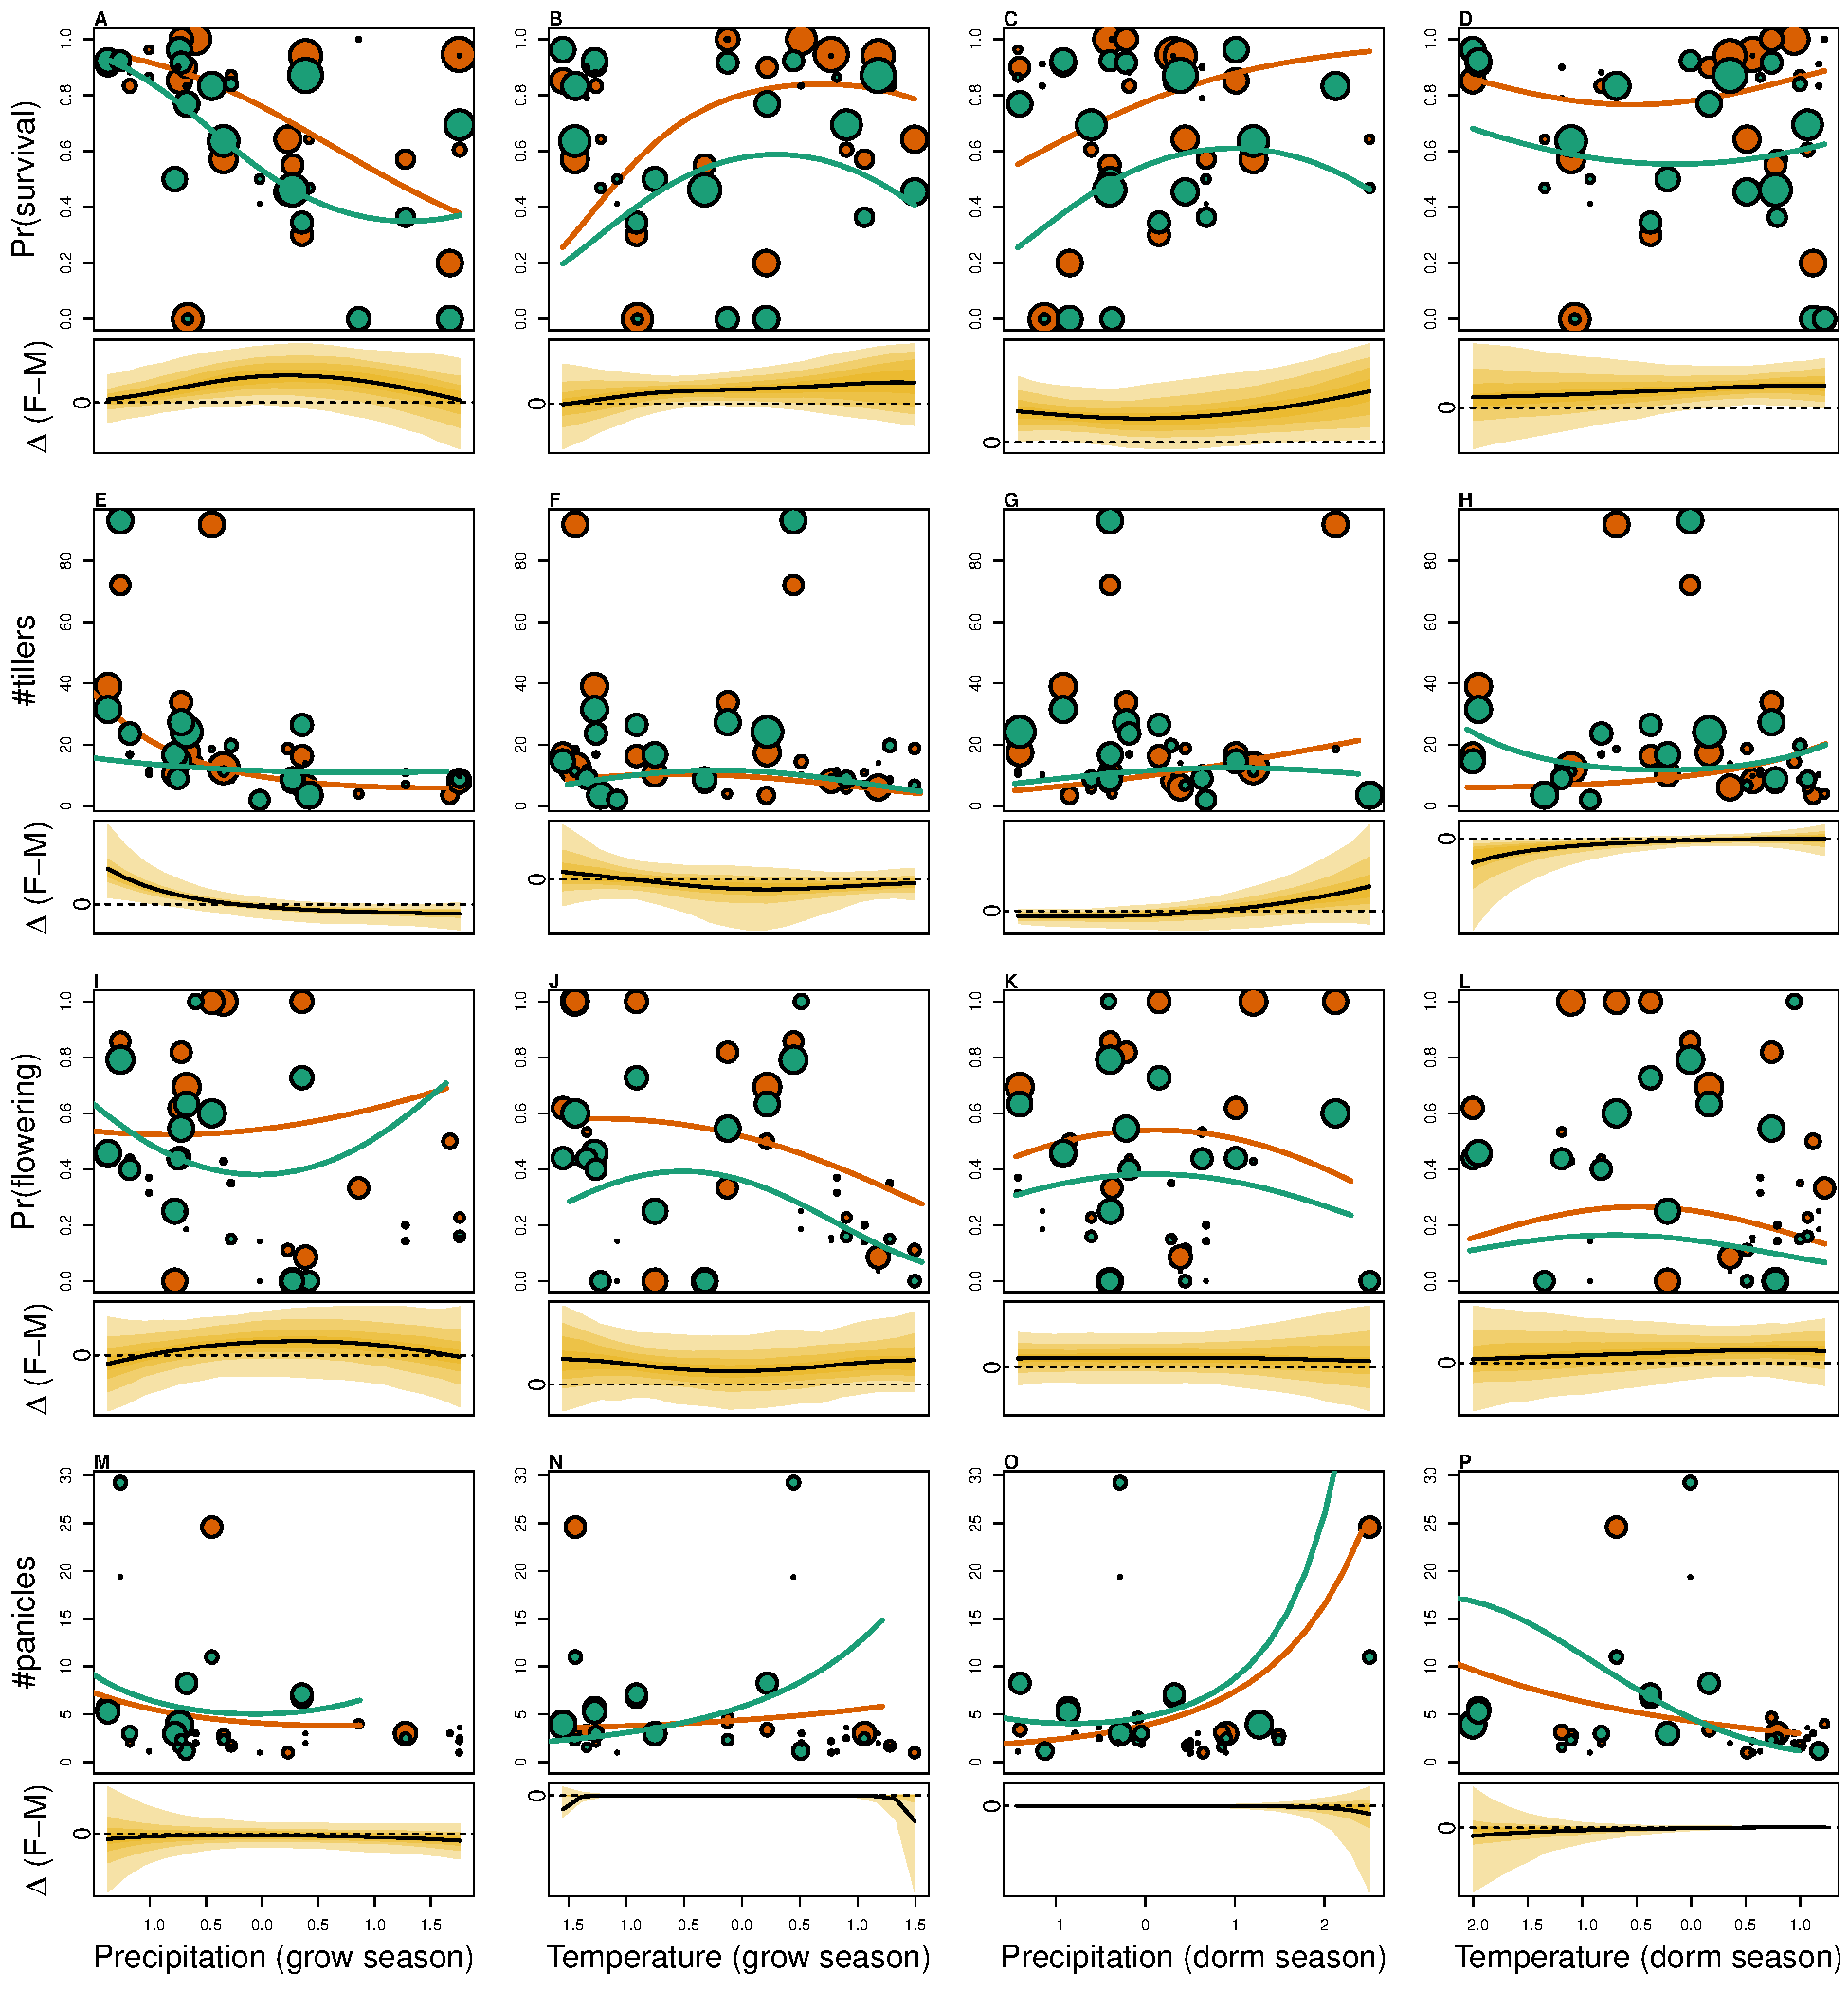
\includegraphics[width=0.95\linewidth]{Figures/vital_rates.pdf}
  \caption{Sex specific demographic response to climate across species range: A--D, inter-annual probability of survival; E--H, inter-annual growth (change in number of tillers); I--L, probability of flowering; M--P, number of panicles produced given flowering. 
  Points show means by site for females (orange) and males (green). 
  Point size is proportional to the sample size of the mean.
  Lines show fitted statistical models for females (orange) and males (green) based on posterior mean parameter values.
  Lower panels below each data panel show the posterior distribution of the difference between females and males as a function of climate (positive and negative values indicate female and male advantage, respectively); dashed horizontal line shows zero difference.}
  \label{fig:vital_rates}
  \end{center}
\end{figure}

\subsection*{Population growth rate response to climate change}

Consistent with the effect of climate on individual vital rate, we also found an effect of seasonal climate on population growth rate. Precipitation and temperature of the growing season decreased the population growth rate, whereas precipitation and temperature of the dormant season increased the population growth rate. Across all sites, the population growth rate was higher than one, suggesting an increase of population over time.

\begin{figure}%[h!]
  \begin{center}
    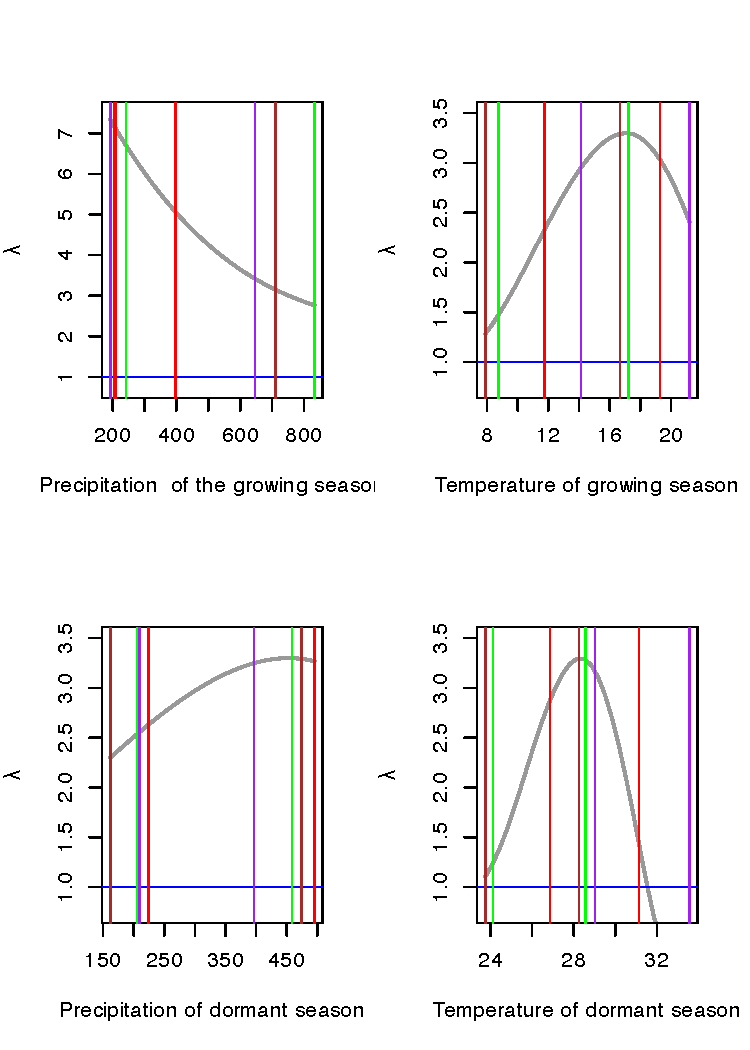
\includegraphics[width=0.95\linewidth]{Figures/all_lambda.pdf}
  \caption{XXX}
  \label{fig:vital_rates}
  \end{center}
\end{figure}


%--------------------------------------------------------------------
\newpage
\section*{Appendix S1: Correspondence }
\renewcommand{\thefigure}{A\arabic{figure}}\setcounter{figure}{0}
\renewcommand{\thetable}{A\arabic{table}}\setcounter{table}{0}
\renewcommand{\theequation}{A\arabic{equation}}\setcounter{equation}{0}
	\begin{figure}[H]
		\centering
		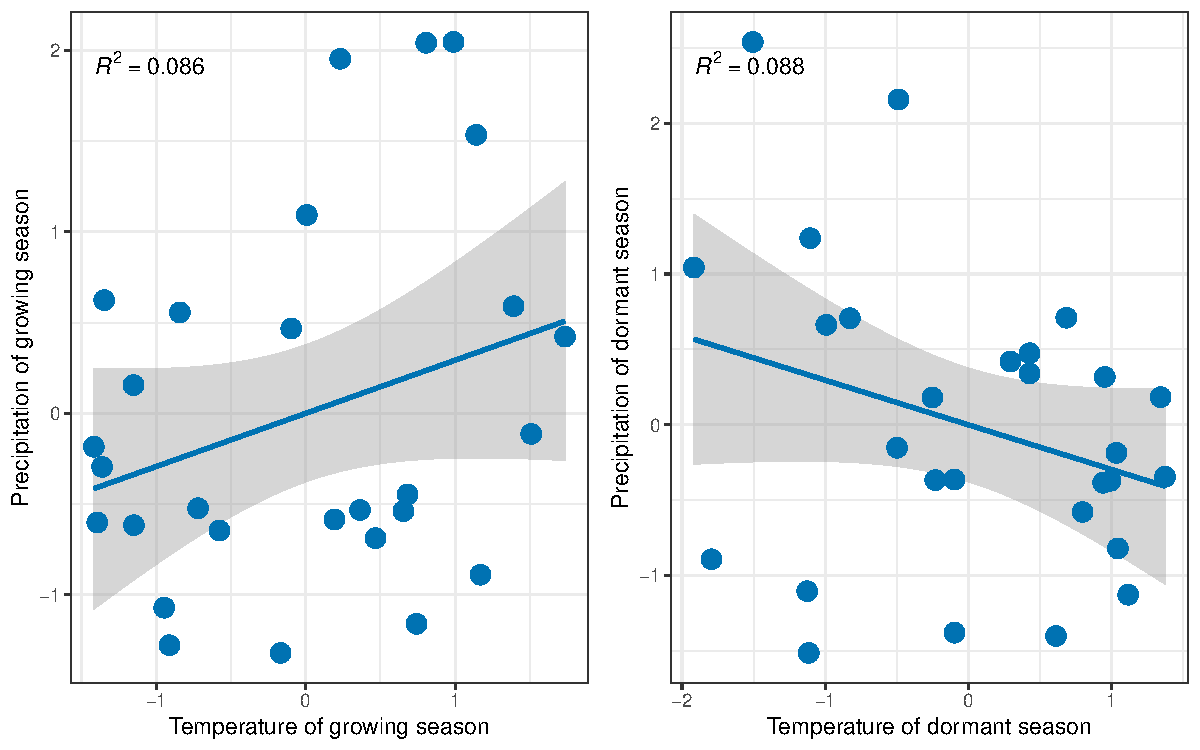
\includegraphics[width = \linewidth]{Figures/Varianceexplained.pdf}
		\caption{\textbf{Relation between precipitation and temperature for each season (growing and dormant).} $R^2$ indicates the value of proportion of explained variance between the temperature and precipitation}
	\end{figure}
	
  \begin{figure}[H]
		\centering
		\includegraphics[scale = 0.5]{Figures/PPCtmax_tmin.pdf}
		\caption{\textbf{Consistency between real data and simulated values suggests that the fitted model accurately describes the data}. Graph shows density curves for the observed data (light blue ) along with the simulated values (dark blue). The first column shows the linear models and the second column shows the 2 degree polynomial models.}
	\end{figure}
	
	
	 \begin{figure}%[h!]
		\centering
		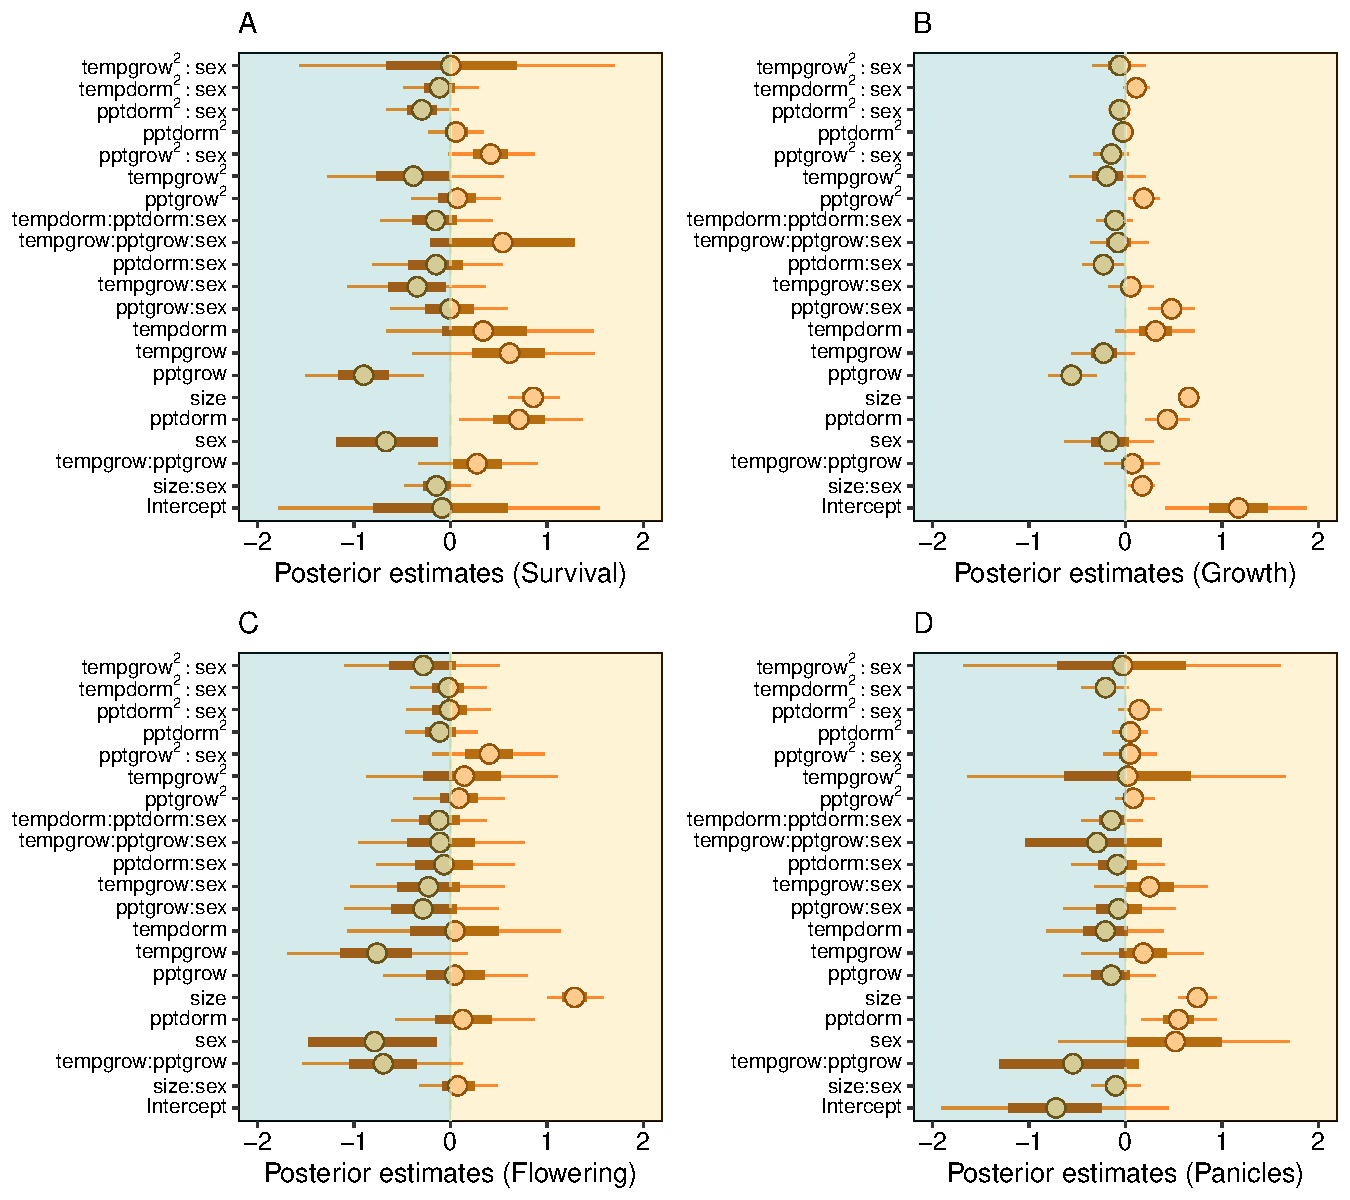
\includegraphics[scale = 4.5]{Figures/Posterior_mean.pdf}
		\caption{\textbf{Posterior mean for each vital rate}. }
	\end{figure}
	

\bibliographystyle{ecology}
\bibliography{Forecasting}
\end{document}
